\documentclass[varwidth]{standalone}
  \usepackage{amsfonts,amsmath,amssymb}
  \usepackage[slovene]{babel}
  \usepackage[utf8]{inputenc}
  \usepackage[T1]{fontenc}
 
  
\usepackage{tikz, verbatim, subcaption}
\usepackage{pgfplots}
\usepackage{mathrsfs}
\usetikzlibrary{arrows}
\usetikzlibrary{arrows.meta, calc, positioning, automata}



\begin{document}

\newcommand*\hight{0.85}

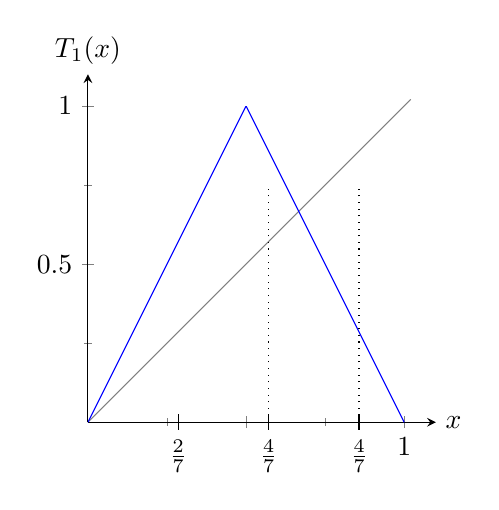
\begin{tikzpicture}
\draw[gray] (0, 0) -- (4.1, 4.1);
\begin{axis}[
width=6cm,height=6cm,
minor tick num=1,
axis y line=middle,
axis x line=middle,
xlabel=$x$,ylabel=$T_1(x)$,
every axis x label/.style={
    at={(ticklabel* cs:1)},
    anchor=west,
},
every axis y label/.style={
    at={(ticklabel* cs:1)},
    anchor=south,
},
xmin=0,
xmax=1.1,
ymin=0,
ymax=1.1
]
	\addplot[blue,mark=none,
		 domain=-0:1,samples=400] 
		{1-max(2*x-1, 1-2*x)};
		
\draw[-latex'] (28.571,0)-- (28.571,57.143);
\draw[-latex'] (28.571,57.143) -- (57.143,57.143);
\draw[-latex'] (57.143,57.143)--(57.143,85.714);
\draw[-latex'] (57.143,85.714)--(85.714,85.714);
\draw[-latex'] (85.714,85.714)--(85.714,28.571);
\draw[-latex'] (85.714,28.571)--(28.571,28.571);

\end{axis}
\filldraw[white] (1.8,-0.5) rectangle (2.3,-0.1);
\draw (1.147,0.1)-- (1.147,-0.1) node[below] {$\frac{2}{7}$};
\draw[dotted] (2.29525,0)-- (2.29525,3);
\draw (2.29525,0.1)-- (2.29525,-0.1) node[below] {$\frac{4}{7}$};
\draw[dotted] (3.4429,0)-- (3.4429,3);
\draw (3.4429,0.1)-- (3.4429,-0.1) node[below] {$\frac{4}{7}$};
\end{tikzpicture}

\end{document}